\documentclass[]{article}
\usepackage{lmodern}
\usepackage{amssymb,amsmath}
\usepackage{ifxetex,ifluatex}
\usepackage{fixltx2e} % provides \textsubscript
\ifnum 0\ifxetex 1\fi\ifluatex 1\fi=0 % if pdftex
  \usepackage[T1]{fontenc}
  \usepackage[utf8]{inputenc}
\else % if luatex or xelatex
  \ifxetex
    \usepackage{mathspec}
  \else
    \usepackage{fontspec}
  \fi
  \defaultfontfeatures{Ligatures=TeX,Scale=MatchLowercase}
\fi
% use upquote if available, for straight quotes in verbatim environments
\IfFileExists{upquote.sty}{\usepackage{upquote}}{}
% use microtype if available
\IfFileExists{microtype.sty}{%
\usepackage{microtype}
\UseMicrotypeSet[protrusion]{basicmath} % disable protrusion for tt fonts
}{}
\usepackage{hyperref}
\hypersetup{unicode=true,
            pdftitle={Liver cancer},
            pdfborder={0 0 0},
            breaklinks=true}
\urlstyle{same}  % don't use monospace font for urls
\usepackage{longtable,booktabs}
\usepackage{graphicx,grffile}
\makeatletter
\def\maxwidth{\ifdim\Gin@nat@width>\linewidth\linewidth\else\Gin@nat@width\fi}
\def\maxheight{\ifdim\Gin@nat@height>\textheight\textheight\else\Gin@nat@height\fi}
\makeatother
% Scale images if necessary, so that they will not overflow the page
% margins by default, and it is still possible to overwrite the defaults
% using explicit options in \includegraphics[width, height, ...]{}
\setkeys{Gin}{width=\maxwidth,height=\maxheight,keepaspectratio}
\IfFileExists{parskip.sty}{%
\usepackage{parskip}
}{% else
\setlength{\parindent}{0pt}
\setlength{\parskip}{6pt plus 2pt minus 1pt}
}
\setlength{\emergencystretch}{3em}  % prevent overfull lines
\providecommand{\tightlist}{%
  \setlength{\itemsep}{0pt}\setlength{\parskip}{0pt}}
\setcounter{secnumdepth}{0}
% Redefines (sub)paragraphs to behave more like sections
\ifx\paragraph\undefined\else
\let\oldparagraph\paragraph
\renewcommand{\paragraph}[1]{\oldparagraph{#1}\mbox{}}
\fi
\ifx\subparagraph\undefined\else
\let\oldsubparagraph\subparagraph
\renewcommand{\subparagraph}[1]{\oldsubparagraph{#1}\mbox{}}
\fi

\title{\protect\hypertarget{ux5fhfngqw9yg5rj}{}{}Liver cancer}
\date{}

\begin{document}
\maketitle

In this section, we will describe the anatomical properties of the liver
and the major public health problem caused by liver cancers. This
section allows us to see the potential value brought by our work
regarding the treatment of liver cancer.

After a small introduction about the different types of liver cancers,
we will focus on the most common primary one: the Hepatocellular
Carcinoma. We will review its risk factors, and the way it develops in
the liver, before exposing the different invasive or non-invasive ways
to establish a clear diagnosis of the disease. Finally we present the
different staging systems and treatments available to provide the better
chance of survival to the diseased patients. A precise description of
the different stages of the disease and the subsequent pathological
changes is necessary in order to understand how our work can further be
incorporated in the clinical practice.

The liver is a key organ in the human body, responsible for the
synthesis of several proteins, and playing a major role during the
digestion, particularly with the production of bile that is further
stored in the gallbladder. It is also essential for the breakdown of
numerous hormones, and it has a central position in the human blood flow
system with its unique dual blood supply, being one of the 3 only portal
systems of the human body and the only venous one.

Being a key organ, the liver can suffer from various pathologies, which
include liver cancer, that is now considered as a major public health
challenge with its high incidence and mortality rates. In their latest
statistical report, the World Health Organization ranked it as the fifth
cancer type in terms of incidence with about 841,000 new cases annually,
and as the fourth cause of cancer-related deaths worldwide, with about
782,000 annual deaths. Mortality and incidence rates are between 2 and 3
times higher among men than women in most regions of the world, making
it the second type of cancer in terms of deaths for males.
{[}\textbf{Bray et al. 2018}{]}\\
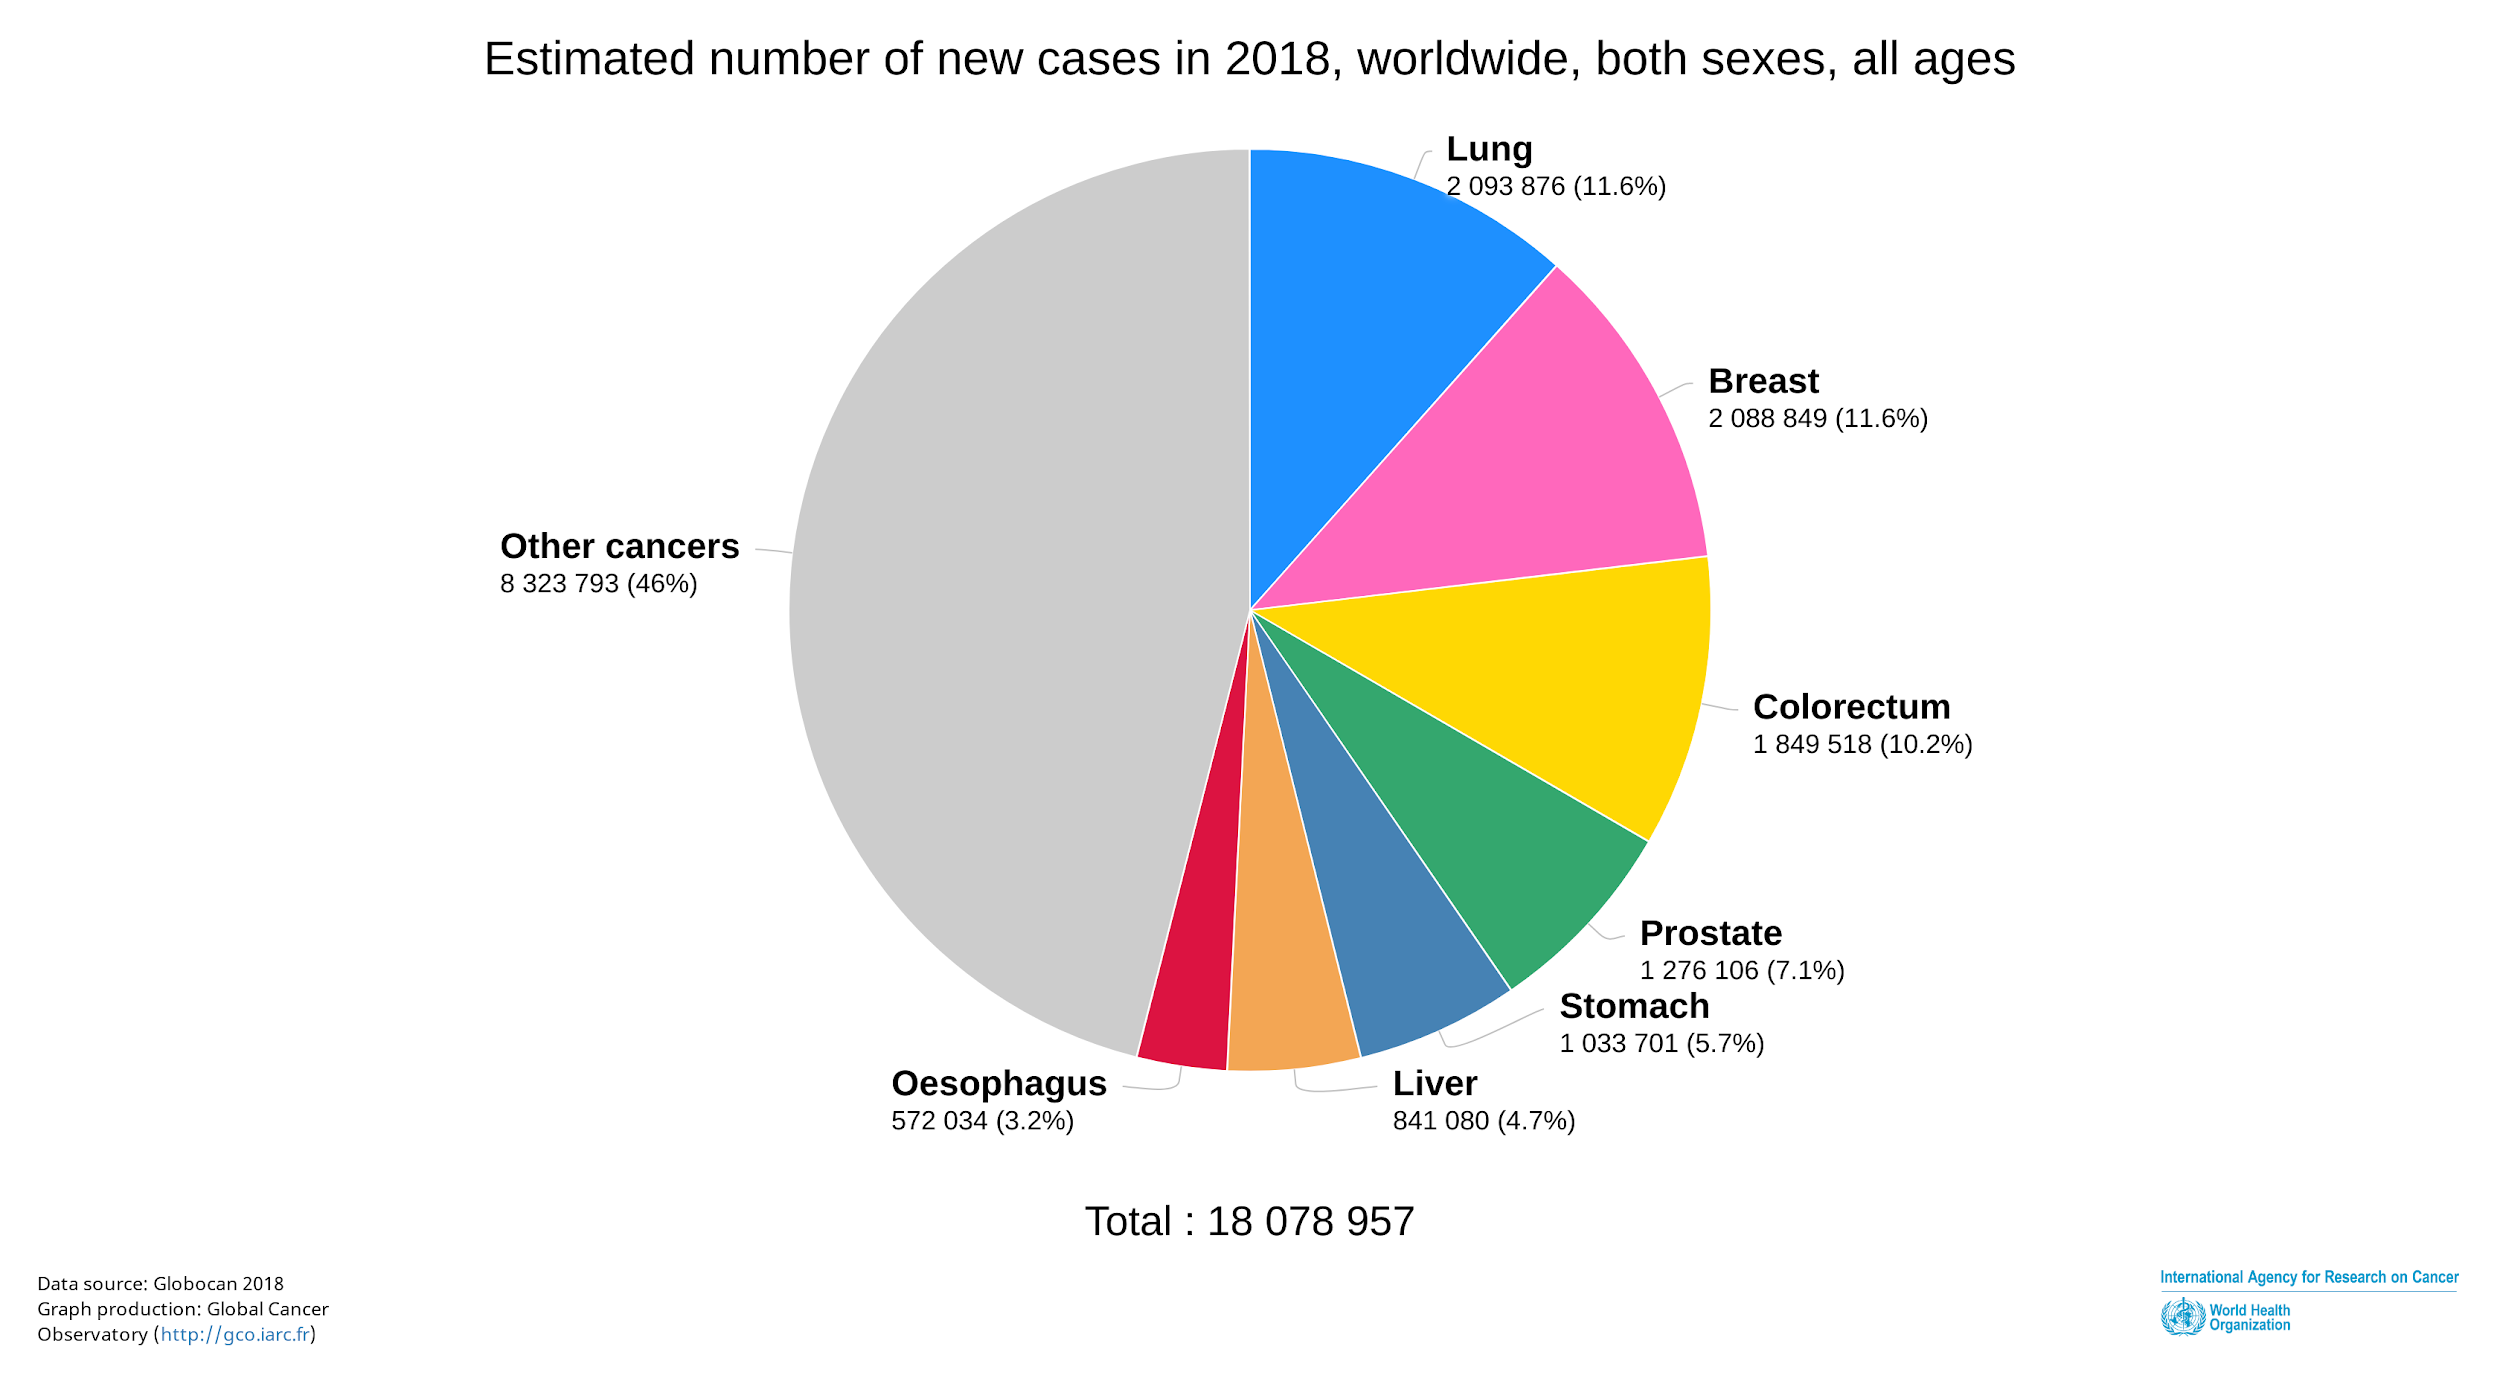
\includegraphics[width=6.25187in,height=3.45313in]{./images/media/image15.png}

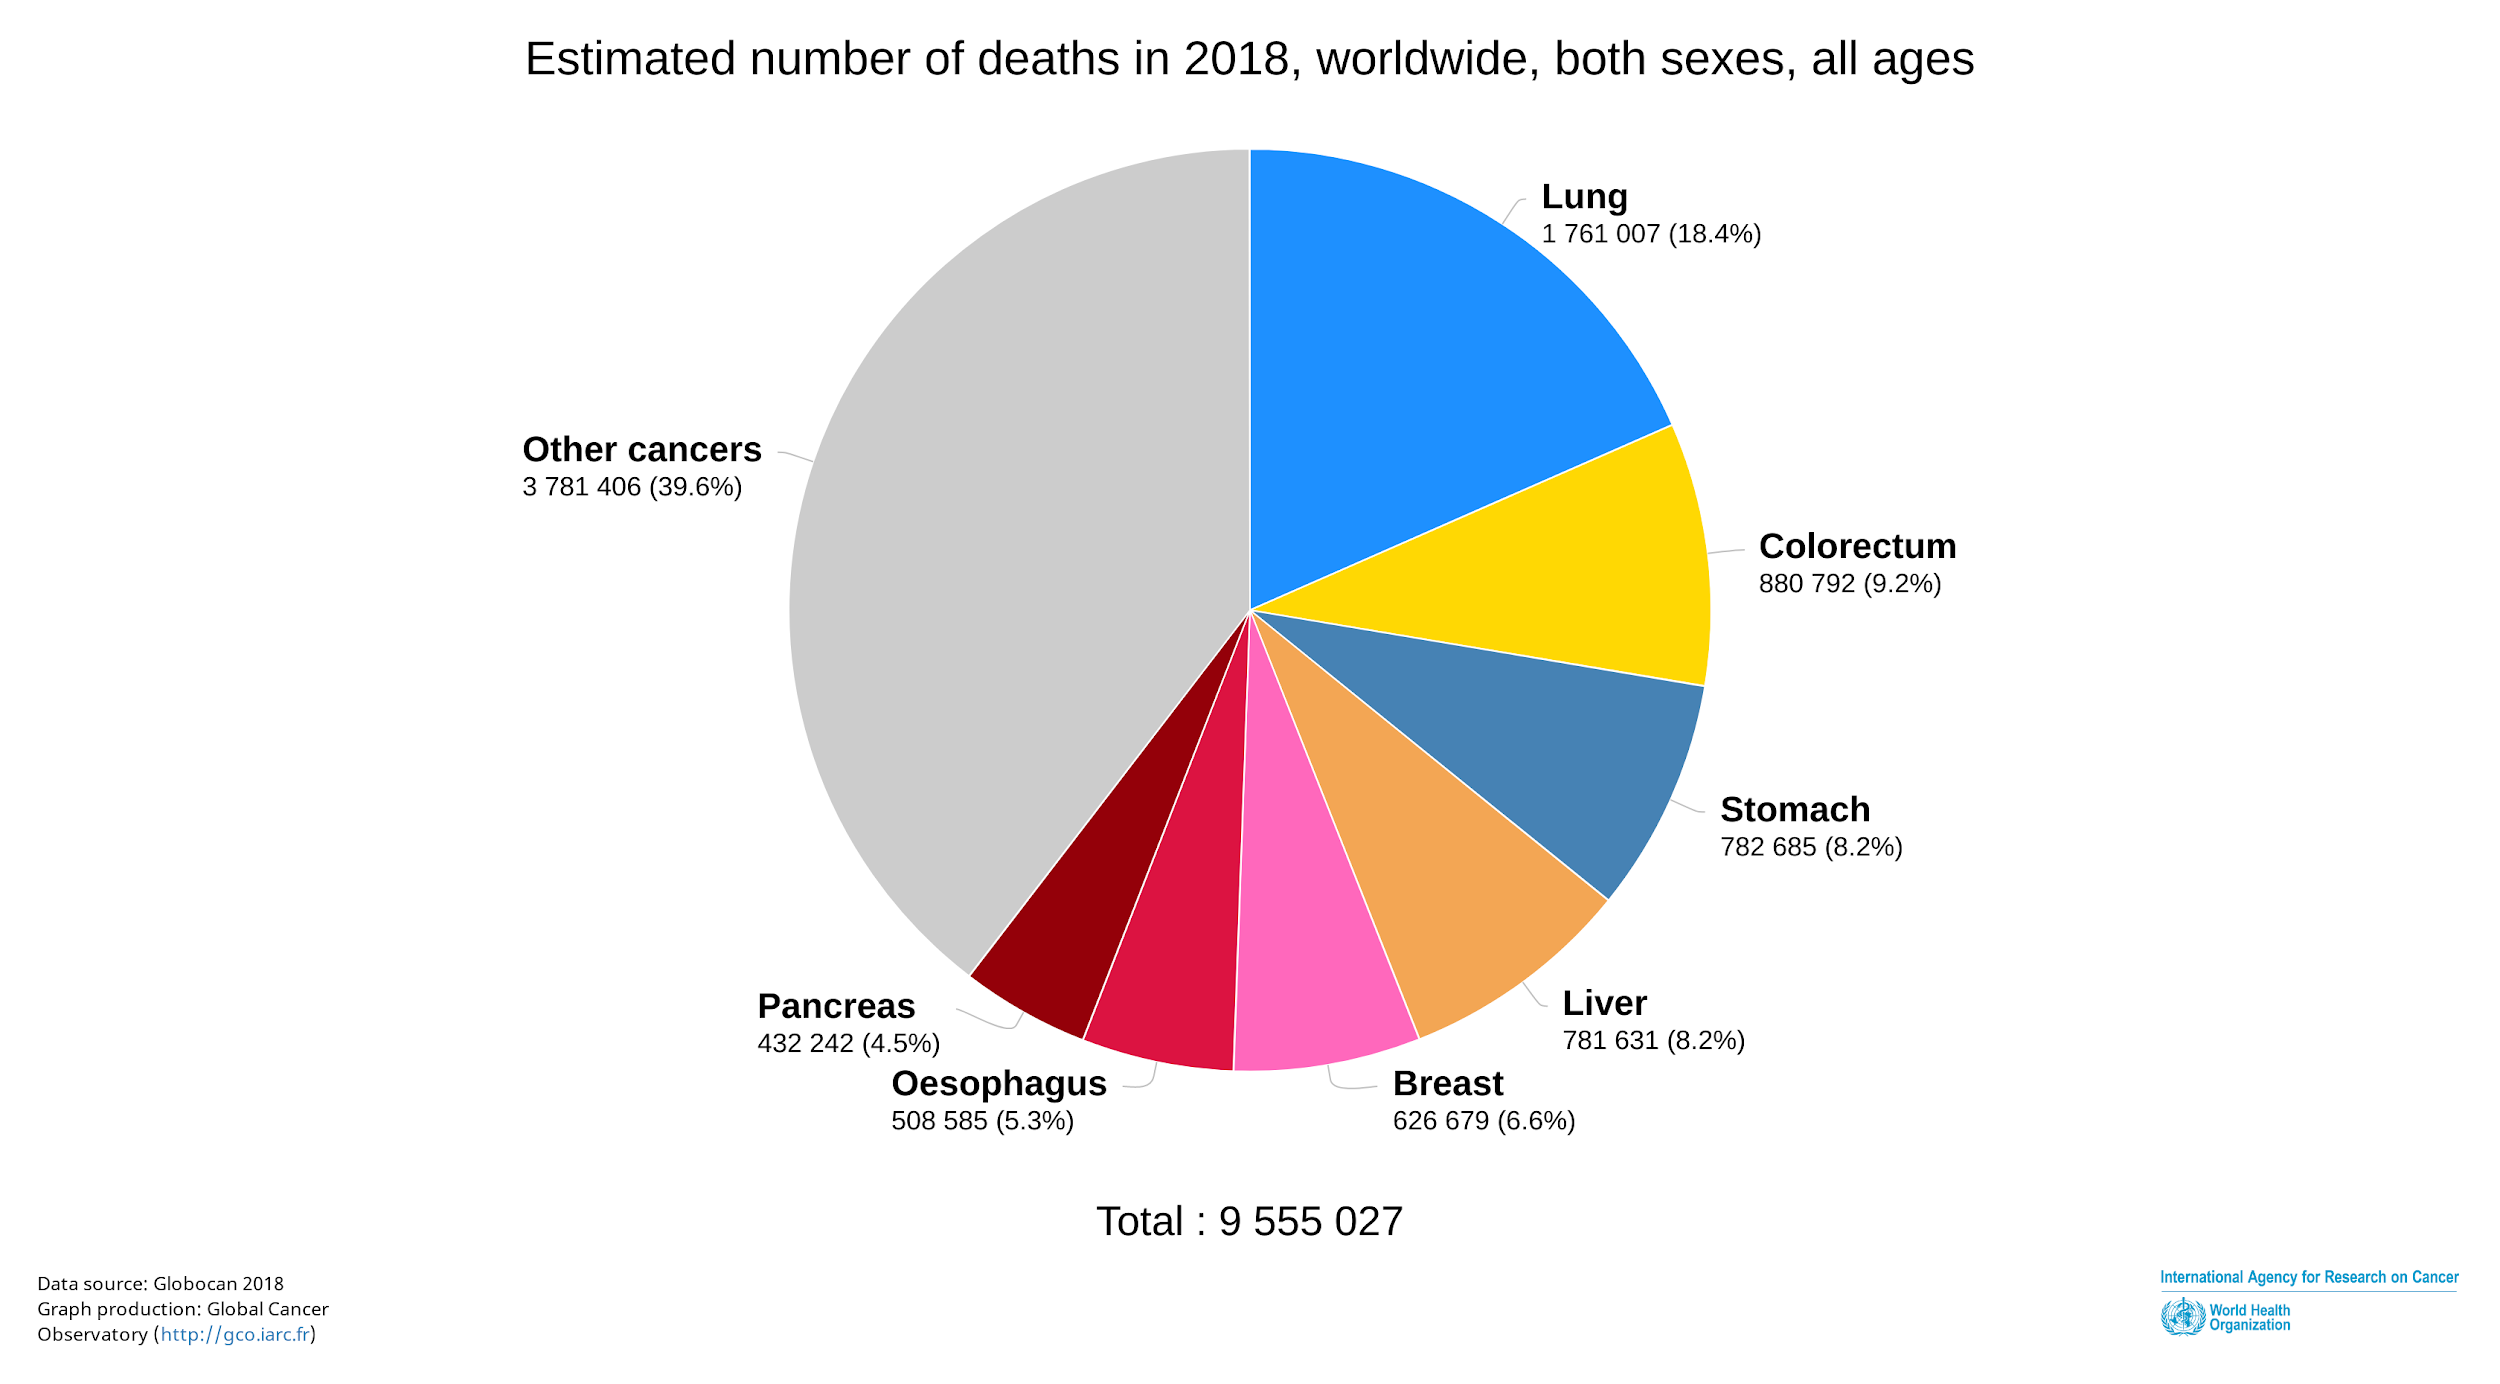
\includegraphics[width=6.26046in,height=3.46354in]{./images/media/image14.png}

The liver cancer can either be referred to as primary, meaning that it
is originally growing in the liver itself, or as secondary, in case of
extrahepatic cancers that metastases in the liver.

In case of metastases, cancerous cells often originate from the lung,
the breast, and some parts of the digestive system, such as the colon,
with the colorectal cancer being the main source of extrahepatic
metastases. {[}\textbf{ref Hoyer et al. 2012, Sahani et al. 2014}{]}

Even though secondary liver cancers are more frequent than primary ones,
we have decided to focus on the latter to analyze the entire process
from the appearance of the malignant cells to the physiological changes.
Indeed, analyzing secondary liver cancers requires a complete
understanding of the alterations in the primary site that led to it.

Primary liver cancers comprise hepatocellular carcinoma (\emph{HCC}),
intrahepatic cholangiocarcinoma (\emph{iCCA}), mixed hepatocellular
cholangiocarcinoma (\emph{HCC-CCA}) and other rare tumors, notably
fibrolamellar HCC (\emph{FLC}) and pediatric neoplasm hepatoblastoma
{[}\textbf{ref Sia et al. 2017 + ref 4-5}{]}.

HCC accounts for nearly 90\% of primary liver cancers, with the highest
incidence in Asia and in the Sub-Saharan countries, mainly due to the
high prevalence of hepatitis B virus (\emph{HBV}) {[}\textbf{ref Sia et
al. 2017 + ref 6}{]}. The second most common one is \emph{iCCA}, with a
noticeable high incidence in Southeast Asian countries, and mainly
developed in patients with primary sclerosing cholangitis (\emph{PSC}),
biliary duct cysts, hepatolithiasis, or parasitic biliary infestation
with flukes. {[}\textbf{ref Sia et al. 2017 + ref 13}{]}.

The high incidence of \emph{HCC} leads us to focus our research work on
this specific cancer type. We will now detail its risk factors,
development, diagnosis methods and treatment techniques.

\section{Hepatocellular Carcinoma}\label{hepatocellular-carcinoma}

\subsection{Risk factors}\label{risk-factors}

The main reason leading to \emph{HCC} is the cirrhotic status of the
liver, but its development is often related to the presence of other
chronic liver diseases.

Its incidence is heterogeneous worldwide because of the variable
prevalence of risk factors: most cases occurring in sub-Saharan Africa
and eastern Asia are associated with \emph{HBV} and aflatoxin B1
exposure. In the USA, Europe and Japan, Hepatitis C (\emph{HCV}) and the
excessive alcohol consumption are the main risk factors {[}\textbf{ref
Fornet et al. 2019}{]}.

Other risk factors include the presence of non alcoholic-fatty liver
disease (\emph{NAFLD}), obesity and diabetes {[}\textbf{ref Marengo et
al. 2016}{]}.

\emph{NAFLD} was defined about 20 years ago, and regroups a spectrum of
progressive liver diseases that encompasses simple steatosis,
nonalcoholic steatohepatitis (\emph{NASH}) and ultimately cirrhosis
{[}\textbf{ref Marengo et al. 2016}{]}. It has been identified as the
underlying cause of patients presenting with \emph{HCC} unrelated to
virus and alcohol {[}\textbf{ref 3 of} \textbf{Marengo et al}{]}.
Several other studies confirmed that \emph{NAFLD} is a risk factor for
patients with either noncirrhotic liver {[}\textbf{ref 33, 30 of}
\textbf{Marengo et al}{]} or cirrhotic liver {[}\textbf{ref 36, 64, 70
of} \textbf{Marengo et al}{]}.

Obesity has been established as a risk factor for several types of
cancer, including liver cancer, and a study on 900,000 American adults
reported a mortality rate five times higher in patients with a body mass
index of 35 kg/m² compared to the group with a normal BMI {[}\textbf{ref
1 of Marengo et al.}{]}. Several other studies were conducted to show
the relation between HCC and obesity in the UK, Korea, Sweden, Taiwan
and also a multicentric European study {[}\textbf{ref 10, 11, 12, 16, 14
of Marengo et al.}{]}.

Diabetes has also been identified as an independent risk factor for HCC
{[}\textbf{ref Fornet et al. 2018}{]}, especially types 2 diabetes
{[}\textbf{ref 21, 19, 18, 22, 17 of Marengo et al.}{]}

\subsection{Development}\label{development}

\subsubsection{Cells of origin of liver
cancer}\label{cells-of-origin-of-liver-cancer}

The basic hepatic cells are divided into parenchymal (hepatocytes, which
constitute between 60 and 80\% of the total liver mass, and
cholangiocytes as depicted in the figure below) and non-parenchymal
cells (fibroblasts, stellate cells, Kupffer cells, and endothelial
cells) {[}\textbf{ref Sia et al. 2017}{]}.

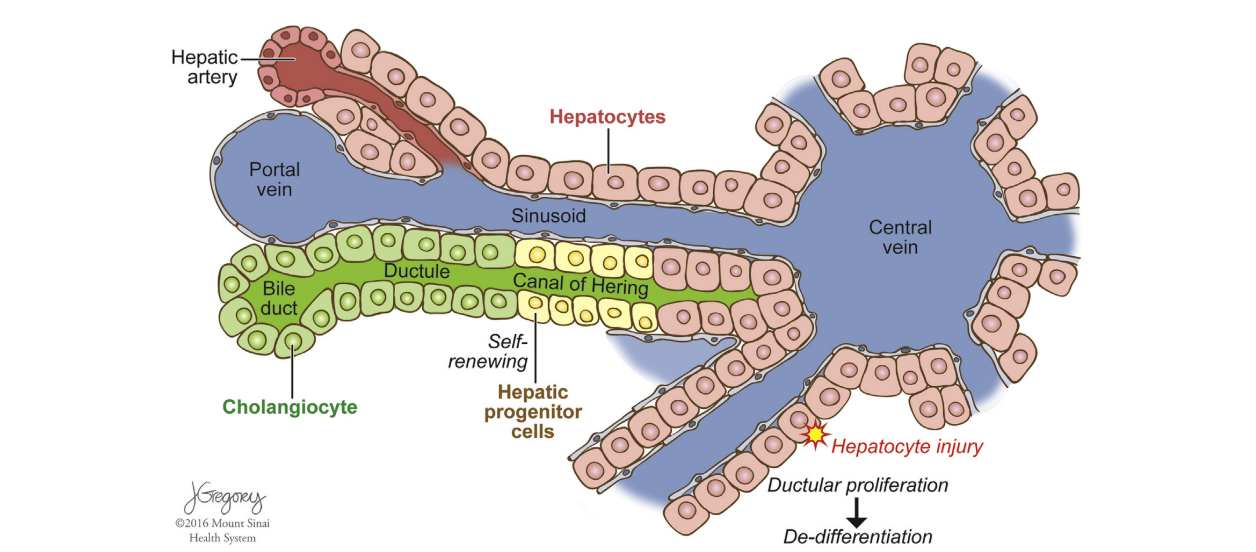
\includegraphics[width=6.26772in,height=2.75000in]{./images/media/image7.png}

The two main primary liver cancers types, \emph{HCC} and \emph{iCCA}
have been considered to be distinct tumors that originate from specific
cell populations. Nonetheless, they have recently been recognized as
subtypes of a continuous spectrum of diseases. Therefore, several
hypotheses exist about the cells of origin of the different primary
liver cancer {[}\textbf{ref Sia et al. 2017}{]}.

One of them suggests that liver tumors can be generated by hepatic
progenitor cells, since during liver development, both hepatocytes and
cholangiocytes both arise from a common progenitor as depicted below.
However, both tumor subtypes can also arise distinctly from mature
parenchymal cells {[}\textbf{ref Sia et al. 2017}{]}.

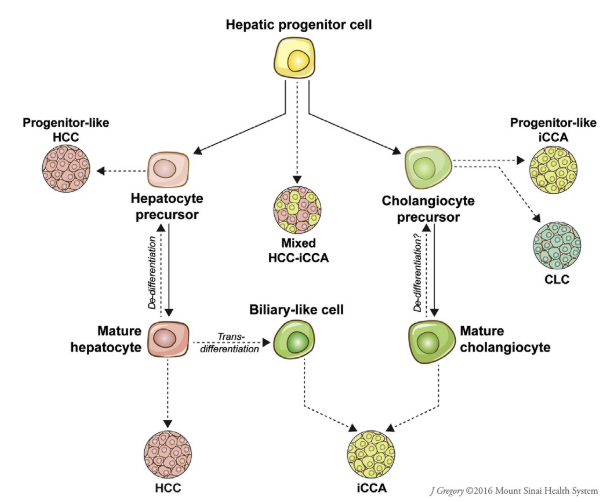
\includegraphics[width=4.02101in,height=3.28628in]{./images/media/image6.png}

This latest hypothesis is the one that we will describe in the
following, and we will focus specifically on the development of
\emph{HCCs}.

\subsubsection{Hepatocarcinogenesis}\label{hepatocarcinogenesis}

The main process behind the evolution of \emph{HCC} is called
\emph{hepatocarcinogenesis}, which is\\
defined as the progressive transformation of nonmalignant liver cells
into \emph{HCC}. {[}\textbf{ref Choi et al. 2014}{]}

This transformation from nonmalignant liver cells into \emph{HCC} is not
fully understood, but the chronic inflammation present in the liver
results in cycles of cell injury-death-regeneration, that stimulate
epidemic changes and accumulation of genetic damages {[}\textbf{ref 11,
20-22 of Choi et al.}{]}\\
The high inter and intra-patient heterogeneity that exists for
\emph{HCCs} is explained by the fact that several molecular variants of
\emph{HCC} may be produced, among the patients population, and even
within different regions of the same tumor {[}\textbf{ref 22, 27 of Choi
et al.}{]}\\
The \emph{hepatocarcinogenesis} is outlined by the gradual
de-differentiation of abnormal nodular lesions, as described in the
figure below {[}\textbf{ref 18,19 of Choi et al.}{]} Over time, the more
differentiated surrounding tissues are replaced by the growing less
differentiated ones.

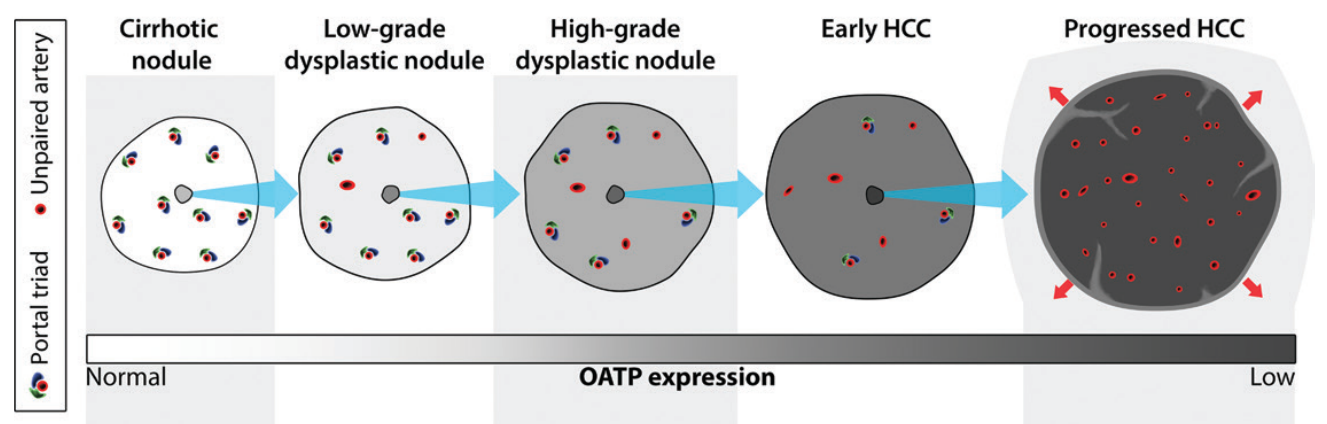
\includegraphics[width=6.26772in,height=2.00000in]{./images/media/image4.png}

It is possible that \emph{HCCs} may arise from malignant cells without
following this process, and without transitioning through histologically
definable intermediate steps the process is then referred to as ``denovo
hepatocarcinogenesis''
{[}\href{https://docs.google.com/document/d/1F5IUt9O-m_2LUTsJQI_7g8W_0PEHzx9hDfyjPOJ7yvo/edit\#heading=h.tuamaz8z9u81}{\textbf{\emph{ref
31 of Choi et al.}}}{]}.

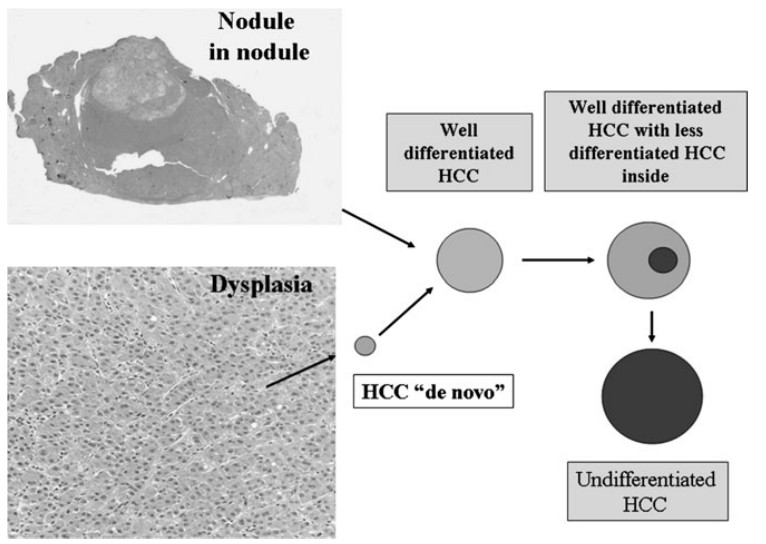
\includegraphics[width=3.34569in,height=2.37022in]{./images/media/image3.png}\\
As depicted in the figure above, hepatocarcinogenesis is composed of
several steps, where each stage presents specific characteristics:

\begin{itemize}
\item
  \begin{quote}
  \emph{Cirrhotic nodules} are well-defined rounded regions of cirrhotic
  parenchyma surrounded by scar tissue and measuring less than 15 mm in
  diameter {[}\textbf{ref 30 of Choi et al.}{]}. Even though they are
  usually considered as non-malignant, \emph{hepatocytes} that they
  contain may develop dysplastic features, thus transforming the
  cirrhotic nodules into a \emph{dysplastic foci} or \emph{nodules}.
  \end{quote}
\item
  \begin{quote}
  \emph{Dysplastic foci} are not identified via in vivo imaging, but may
  be recognized histologically. They are not well understood and may
  develop into \emph{dysplastic nodules}.
  \end{quote}
\item
  \begin{quote}
  \emph{Dysplastic nodules} correspond to nodular lesions that differ
  macro and microscopically from the surrounding parenchyma. They are
  observed in 25\% of cirrhotic livers, and can be classified into
  low-grade (that appear like cirrhotic nodules) or high-grade (more
  similar to well-differentiated \emph{HCCs})
  \end{quote}
\item
  \begin{quote}
  \emph{Early HCCs} grow gradually by replacing the parenchyma, unlike
  apparent progressed \emph{HCCs} that displace or destroy the liver
  parenchyma. During their evolution, they tend to surround structures
  like portal tracts or central veins without destroying them.\\
  They are microscopically indistinguishable from high-grade dysplastic
  nodules, since they tend to be vaguely nodular without having capsules
  nor distinct margins.\\
  Even if they are considered as ancestors of progressed \emph{HCCs}
  {[}\textbf{ref 19 of Choi et al.}{]}, their progression rate is not
  clearly defined {[}\textbf{ref 39 of Choi et al.}{]}\\
  \emph{TO REMOVE:} \emph{As described later, the hepatobiliary phase MR
  imaging is one of the only imaging modality that tends to show promise
  for detecting them.}
  \end{quote}
\item
  \begin{quote}
  \emph{Progressed HCCs} are generally separated between those measuring
  less than 2cm and those larger than 2cm.
  \end{quote}

  \begin{itemize}
  \item
    \begin{quote}
    Those smaller than 2cm tend to be nodular with a well-defined
    margin. They are different from early \emph{HCCs} in the way that
    they grow by expanding into and compressing the adjacent parenchyma.
    They tend to be histologically moderately differentiated in the vast
    majority of the cases, and are associated with vascular invasion and
    intrahepatic metastasis {[}\textbf{ref 19 of Choi et al.}{]}
    \end{quote}
  \item
    \begin{quote}
    The large progressed \emph{HCCs} tend to have a more aggressive
    biological behavior, and are associated with a higher histological
    grade, with a higher presence of vascular invasion and metastasis.\\
    They are histologically composed of poorly differentiated or
    undifferentiated cancer cells that spread into the surrounding
    sinusoids, thus often characterized by an ill-defined boundary
    {[}\textbf{ref 4 -11 of Choi et al.}{]}
    \end{quote}
  \end{itemize}
\item
  \begin{quote}
  \emph{Multifocal HCC} can be the result of a synchronous development
  of several independent liver tumors originating from a primary tumor
  {[}\textbf{ref 11 of Choi et al.}{]}, knowing that patients with
  \emph{HCC} are at higher risk of developing new tumors.
  \end{quote}
\end{itemize}

These several steps defining hepatocarcinogenesis are most of the time
accompanied by some pathophysiological alterations:

\begin{itemize}
\item
  \begin{quote}
  \emph{Angiogenesis}: that is histologically characterized by the
  development of unpaired (or nontriadal) arteries as depicted in the
  Figure ``hepatocarcinogenesis steps'' and the transformation of
  hepatic sinusoids into continuous capillaries\textbf{,} a.k.a
  ``sinusoidal capillarization'' {[}\textbf{ref 28-29 of Choi et
  al.}{]}\\
  Besides these changes, the portal tracts, containing both the
  non-tumoral hepatic arteries and the portal veins, progressively
  decrease {[}\textbf{ref 47 of Choi et al.}{]}.\\
  Whereas the portal inflow to the nodule diminishes, the formation of
  unpaired arteries causes an increase in arterial flow {[}\textbf{ref
  28-29 of Choi et al.}{]}. This difference in blood inflow is such that
  we observe a total inversion of tendency during the
  hepatocarcinogenesis, with a decrease of arterial flow accompanied by
  a preservation of portal venous flow in the early phases, and a
  decrease of portal blood flow with an increase of arterial flow in the
  later phases, as depicted in the figure below:\\
  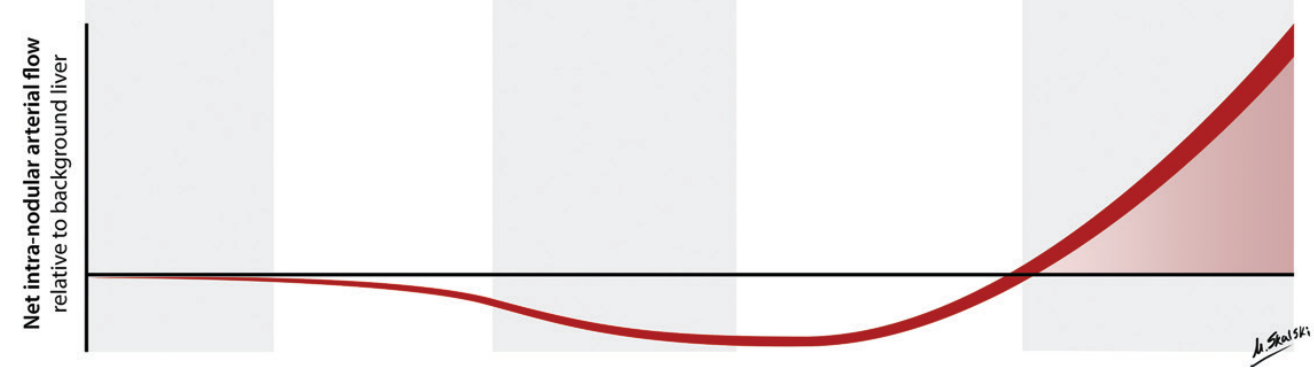
\includegraphics[width=5.77121in,height=1.60796in]{./images/media/image2.png}
  \end{quote}
\item
  \begin{quote}
  \emph{Venous drainage}: During hepatocarcinogenesis, the way the blood
  is drained by the lesions is subject to modifications as depicted in
  the figure below {[}\textbf{ref Kitoa 2009}{]}.
  \end{quote}
\end{itemize}

\begin{quote}
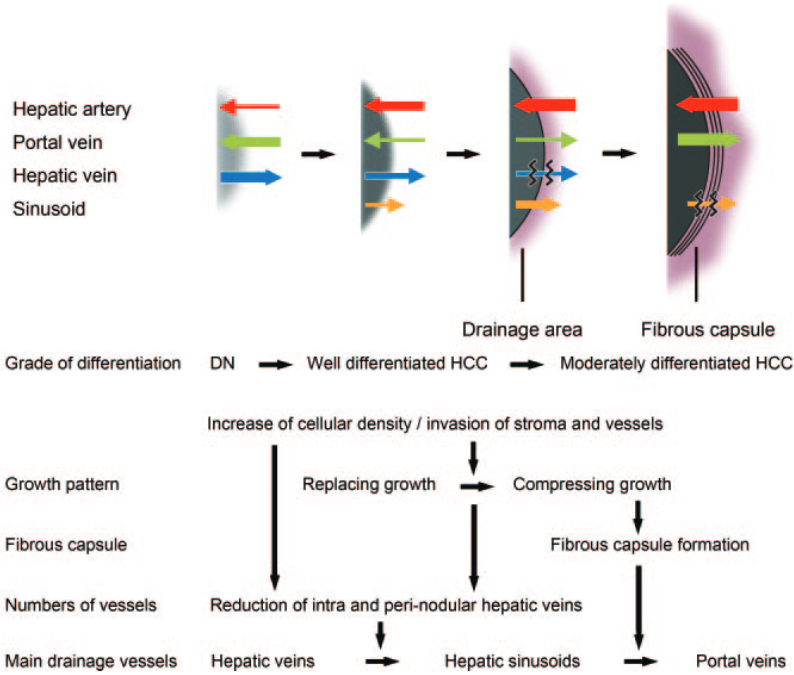
\includegraphics[width=5.19078in,height=4.41133in]{./images/media/image10.png}\\
First, the blood is evacuated via hepatic veins, then sinusoids are used
and replace the hepatic veins that start to be blocked. Later during the
process, the sinusoids start to collapse and the blood cannot be
delivered through this way, therefore, the only remaining way is through
the portal veins {[}\textbf{ref 50-51 of Choi et al.}{]}.

This change along the disease progression may explain the phenomenon of
corona enhancement, which appears mainly on progressed hypervascular
\emph{HCC}, and which referred to an enhancement of the peritumoral
parenchyma starting a few seconds after the enhancement of the tumor.
Worth noting that early \emph{HCCs} are not concerned by this phenomenon
{[}\textbf{ref 52 of Choi et al.}{]}
\end{quote}

\begin{itemize}
\item
  \begin{quote}
  \emph{Tumor Capsule and Fibrous Septa}: are observed in about 70\% of
  progressed nodular \emph{HCCs} {[}\textbf{ref 42 of Choi et al.}{]},
  with a capsule consisting of two distinct layers.\\
  Some studies have shown that tumors with an intact capsule were
  associated with a lower recurrence rate than those without (tumors of
  similar size), suggesting that the capsule may retard the tumor
  dissemination, especially the tight inner layer that might act as a
  physical barrier {[}\textbf{ref 57 of Choi et al.}{]}\\
  Even though advanced \emph{HCCs} with an intact capsule have a more
  favorable prognosis than \emph{HCCs} of the same size without any
  capsule, they have a worse prognosis than early \emph{HCCs} that are
  unencapsulated {[}\textbf{ref 59 of Choi et al.}{]}
  \end{quote}
\item
  \begin{quote}
  \emph{Fat content}: It has been demonstrated that hepatocytes may
  accumulate fat during the early phases of hepatocarcinogenesis,
  causing the tumors to be more steatotic.\\
  This steatosis is highly frequent for early \emph{HCCs} of about 1.5
  cm in diameter, but decreases when the size and the grade of the tumor
  increases. This might probably be because unpaired arteries become
  more developed once the tumor progresses, resolving ischemic
  conditions, and provoking the regression of steatosis {[}\textbf{ref
  47, 61 of Choi et al.}{]}
  \end{quote}
\item
  \begin{quote}
  \emph{Iron content} may accumulate early in the process of
  hepatocarcinogenesis, noticeable essentially in low or high grade
  dysplastic nodules {[}\textbf{ref 33 of Choi et al.}{]}. In the later
  stages, hepatocytes become resistant to iron accumulation due mainly
  to the utilization of iron by neoplastic cells and a higher cellular
  proliferation, thus early and progressed HCCs are often iron free
  {[}\textbf{ref 65 of Choi et al.}{]}.
  \end{quote}
\item
  \begin{quote}
  \emph{Diminution in the expression of OATP Transporters}. Some of
  these transporters belonging to the \emph{OATP} (\emph{Organic anionic
  transporting polypeptides)} group are thought to be responsible for
  the uptake of two hepatobiliary-specific gadolinium-based contrast
  agents, namely the gadoxetate disodium and gadobenate dimeglumine.\\
  Their expression level tends to be inversely proportional to the
  advancement of the disease {[}\textbf{ref 67, 69 of Choi et al.}{]}
  \end{quote}
\end{itemize}

The different alterations are often the results of early or more
advanced stages of hepatocarcinogenesis. They can appear individually or
can be combined within the same tumor.

However, the \emph{HCC} can often later spread either intra or
extra-hepatically:

\begin{itemize}
\item
  \begin{quote}
  \emph{Intrahepatic metastasis:} corresponds to one of the most
  important spread mechanisms of progressed \emph{HCCs}, and occurs
  mainly when malignant cells enter portal venules that drain the
  primary tumor, before spreading into the surrounding parenchyma.\\
  These metastases around the primary tumor in the form of small
  satellites, and are located within its venous drainage area
  {[}\textbf{ref 74 of Choi et al.}{]}. Even though malignant cells can
  easily invade vessels, extrahepatic metastases occurring in organs
  such as the lungs, the lymph nodes, the bones or the adrenal glands,
  are late manifestations of the disease {[}\textbf{ref 6, 11 of Choi et
  al.}{]}
  \end{quote}
\item
  \begin{quote}
  \emph{Vascular invasion}: is a late manifestation of
  hepatocarcinogenesis, affecting mainly the progressed \emph{HCCs}
  {[}\textbf{ref 77 of Choi et al.}{]}, and allows a distinction between
  primary and secondary liver cancers which uncommonly present an
  invasion of intrahepatic vessels {[}\textbf{ref 76 of Choi et
  al.}{]}\\
  These invasions are either classified as micro or macroscopic, and
  usually are accompanied by a poor prognosis, as they provide a way for
  cancerous cells to propagate in the liver or systemically. Moreover,
  patients suffering from cancers with vascular invasion tend to have a
  higher recurrence rate after ablation, resection and transplantation,
  therefore, vascular invasion is often considered as a contraindication
  for these specific treatments {[}\textbf{ref 81 of Choi et al.}{]}\\
  Furthermore, another alteration, called ``\emph{Tumor Capsule
  invasion}'' may increase the risk of vascular invasion, as \emph{HCC}
  cells may infiltrate through the tumor capsule into the surrounding
  parenchyma.
  \end{quote}
\end{itemize}

All the changes occurring during hepatocarcinogenesis, leading to a more
or less aggressive tumor, or even to multiple tumors, need to be
assessed as early as possible to provide the best treatment available to
the patient in order to increase its chances of survival.

\subsection{Diagnosis}\label{diagnosis}

\subsubsection{Biopsy}\label{biopsy}

One of the standard ways to determine or confirm the cause and the stage
of liver disease, as well as to inform treatment decisions and establish
prognosis is to perform a \emph{biopsy}.\\
This surgical procedure consists of the sampling of typically one
fifty-thousandth of the liver volume {[}\textbf{ref 1 of Tapper et
al.}{]}.

The sampled tissues are then reviewed by pathologists, who report the
degree of inflammation, steatosis, fibrosis and some other features such
as cellular inclusions. The histological assessment is supported by
clinicians providing the clinical context to complete the histologic
interpretation, and some external blood markers such as the \emph{AFP}
(alpha-fetoprotein) level can be incorporated to attest the presence of
a malignant mass {[}\textbf{ref Bai et al. 2017 - Zaho et al. 2014 -
Heimbach et al. 2017}{]}.

This method however suffers from several limitations. Sampling errors
are common, as reported by a study where laparoscopic biopsy samples,
taken simultaneously from the right and the left lobes of several
patients suffering from HCV, were interpreted as cirrhotic in one lobe
and fibrotic (F3) in the other in almost 15\% of the cases
{[}\textbf{ref 7 of Tapper et al.}{]}. It has also been proven that the
accuracy of both the diagnosis and the staging of the disease highly
depend on the size of the specimen, with misinterpretations when too
small samples are collected {[}\textbf{ref 8 of Tapper et al.}{]}.\\
The interpretation of the samples is very subjective as it has been
proven in some studies, with the estimation of both inflammatory
activity and fat burden that suffered from a high inter and
intraobserver variability {[}\textbf{ref 3 of Tapper et al.}{]}.
Moreover, being a surgical gesture, the biopsy can suffer from adverse
events going from simple pain to death in some rare cases {[}\textbf{ref
2, 10-12 in Tapper et al.}{]}. Finally, they happen to be costly since
they involve an expert gastroenterologist or radiologist, a pathologist,
and need to be performed in facilities with adequate equipment.

Even though biopsy is still used to evaluate the degree of fibrosis or
cirrhosis, primary liver cancers are now most often diagnosed on the
basis of imaging studies alone in clinical practice. Recent advancements
in medical imaging enable the radiologist to discern the cause of focal
liver lesions on the basis of vascularity and physiological features,
especially through multiphasic, contrast-enhanced, cross-sectional
imaging (either computed tomography \emph{CT}, or magnetic resonance
\emph{MR}).

\subsubsection{CT and MR imaging}\label{ct-and-mr-imaging}

As explained previously, hepatocarcinogenesis is a long process that can
render the tumor very aggressive, and the more the disease evolves, the
worse the prognosis will be for the patient, thus an early detection of
HCC is critical to improve the survival of affected patients.

The majority of the current guidelines recommend ultrasonography (US) as
the primary imaging test for surveillance {[}\textbf{ref Choi et al.
2014}{]}. CT and MRI are generally not chosen for surveillance but
recommended by some guidelines when the US is limited due to obesity or
when the risk factors are very high {[}\textbf{ref 13, 14 Choi et al.
2014}{]}.

If the surveillance is positive, the main guidelines advocate in favor
of multiphasic CT and MR with extracellular agents for the non-invasive
diagnosis and staging {[}\textbf{ref 4, 12-14 of Choi et al. 2014}{]}.

Multiphasic CT and MRI can be categorized by the type of contrast agents
used:

\begin{itemize}
\item
  \begin{quote}
  Imaging with extracellular contrast agents permits a diagnosis of
  \emph{HCC} based on the physiological changes in the blood flow
  produced by hepatocarcinogenesis.\\
  Images are typically acquired before (precontrast) and dynamically
  after the injection of a contrast agent.\\
  The contrast agent is generally administered at a rate of 4-6 mL/sec
  for CT and around 2 mL/sec for MRI {[}\textbf{ref 85-86 of Choi et al.
  2014}{]}. The dose is usually adjusted to the body weight, where 1.5-2
  mL/kg to achieve an iodine dose of 525 mg/kg of iodine are
  administered in the case of CT.\\
  Concerning the dynamic contrast enhanced images, three phases are
  typically acquired, namely the late hepatic arterial, the portal
  venous, and the delayed phase:
  \end{quote}

  \begin{itemize}
  \item
    \begin{quote}
    The l\emph{ate hepatic arterial} phase is characterized by the full
    enhancement of the hepatic artery with all its branches and an
    enhancement of the portal vein {[}\textbf{ref Choi et al. 2014}{]}.
    The portal vein is however not supposed to be enhanced by the
    antegrade flow {[}\textbf{ref 87 of Choi et al.}{]}.\\
    This phase is critical for the characterization of hypervascular
    \emph{HCCs}, since it catches the peak arterial enhancement
    of~tumors {[}\textbf{ref 88 of Choi et al.}{]}. The \emph{early
    hepatic arterial} phase is often omitted by the centers as only
    hepatic arteries are enhanced but portal veins are not, which render
    the detection of hypervascular tumors very difficult. One of the
    main problems associated with this acquisition is the difficulty to
    detect the peak arterial perfusion, since fixed delay is often not
    reliable. Some techniques such as contrast agent bolus tracking, or
    the selection of the best image after multiple continuous
    acquisitions may be recommended {[}\textbf{ref 90 of Choi et
    al.}{]}.
    \end{quote}
  \item
    \begin{quote}
    The \emph{portal venous} phase is characterized by an enhancement of
    both hepatic artery (arterial) and portal veins. It is however worth
    noting that the contrast agent still circulates in the body and will
    still be present in hepatic arteries as well (but with a lower
    concentration than for the arterial phases).\\
    The portal venous phase is generally acquired at around 60-80
    seconds after the start of the injection, but no clear guidelines
    are given concerning a precise way to determine the best moment for
    the acquisition of this given phase.
    \end{quote}
  \item
    \begin{quote}
    The \emph{delayed phase} is acquired 3-5 minutes after the injection
    and helps to understand how the liver restores the contrast agent
    back to the rest of the body, especially in case of inhomogeneous
    washout.
    \end{quote}
  \end{itemize}
\end{itemize}

\begin{quote}
Both the \emph{portal venous} and the \emph{delayed} phases are critical
for the characterization of washout and/or capsule appearance, and are
crucial for the differentiation of small \emph{HCCs} from small
\emph{ICCs} {[}\textbf{ref 93-94 of Choi et al.}{]}. Some centers decide
to skip the delayed phase, but it can lead to a loss of information.

\emph{Precontrast images} are useful in case of detection of enhancement
and evaluation of its degree by subtracting the post-contrast image with
the preconstrast one. They are also useful for patients with iron-rich
nodules to detect hyper attenuation before injection of contrast agent,
thus avoiding misinterpretation of arterial phase enhancement.\\
In addition to these classical vascular phases, examinations performed
with MR imaging usually include other phases such as the T1-weighted
in-phase, the T2-weighted fast-spin-echo and some diffusion-weighted
sequences.\\
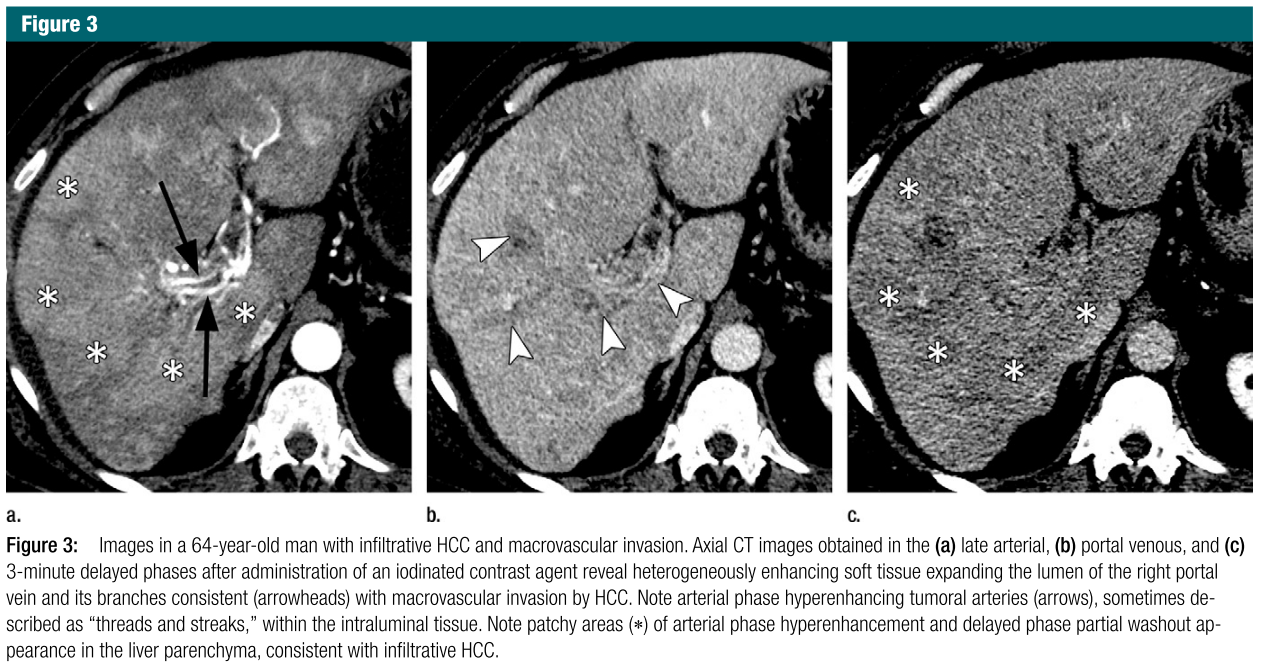
\includegraphics[width=5.67251in,height=2.97760in]{./images/media/image13.png}
\end{quote}

\begin{itemize}
\item
  \begin{quote}
  In order to fully understand the behavior of \emph{HCC} cells, one can
  use extracellular agents as explained above, or use intracellular
  agents. In the latter case, hepatobiliary agents allow a better
  diagnosis through understanding the hepatocellular function in
  addition to the vascularity information. These agents first enhance
  the extracellular space before entering the hepatocytes through the
  OATP specific receptors. To acquire this hepatobiliary phase, which
  can exclusively be obtained on MRI, different agents exist, and they
  mainly differ in their hepatocellular uptake, thus reaching an
  enhancement at different moments. In the exception to the delayed
  phase for some specific agents, the normal phases can be acquired,
  along with some new phases such as the ``transitional phase'', which
  represent a transition from extracellular-dominant to
  intracellular-dominant enhancement {[}\textbf{ref 116 of Choi et
  al.}{]}.\\
  Unlike extracellular agents, the hepatobiliary contrast agents show
  promise for differentiating early \emph{HCCs} and premalignant nodules
  from lower-risk nodules {[}\textbf{ref 31-37 of Choi Part2 et
  al.}{]}.\\
  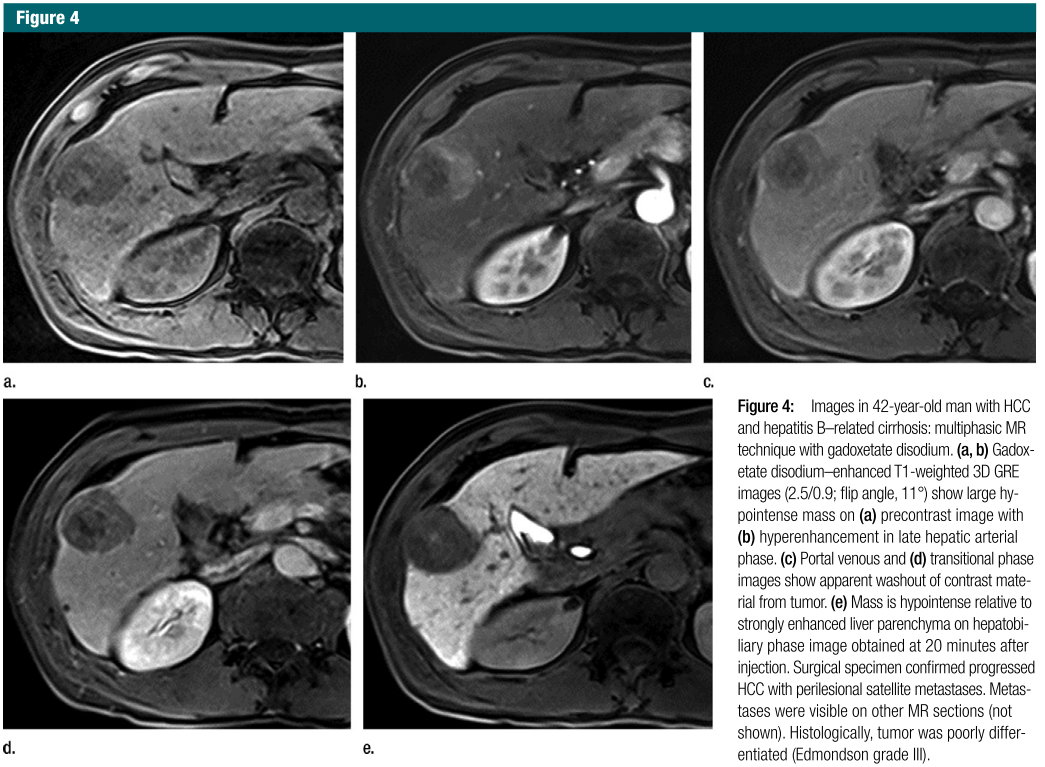
\includegraphics[width=5.62080in,height=4.11678in]{./images/media/image9.png}
  \end{quote}
\end{itemize}

Main advantages of choosing CT over MRI examination is that it is widely
available, rapid, robust and requires less expertise than MRI when
interpreting images. It however exposes patients to radiation doses, and
provides relatively lower soft-tissue contrast than when MRI is used.
MRI permits the assessment of a great number of tissue characteristics,
but is time-consuming, less robust, and prone to artifacts. Even though
MR imaging examination may be preferred at some academic centers, there
is no consensus for recommending this modality over CT in community or
less-specialized centers {[}\textbf{ref Choi et al Part2. 2014 -
Heimbach et al. 2017}{]}.

Therefore, it has been decided to mainly focus our research work on CT
images.

These recent innovations in the medical imaging fields were accompanied
by the creation of several clinical criteria that helped the
radiologists to take decisions concerning the treatment choice,
depending mainly on the characteristics of the tumor.

\subsection{Staging \& Treatment}\label{staging-treatment}

One of the most widely used criteria for the assessment of \emph{HCCs}
is the \emph{BCLC} staging system, recently refined by Llovet et al. in
2008 {[}\textbf{ref Llovet et al.}{]}.

As described in the figure below, the main factors used to build this
staging system rely on the \emph{tumor status}, namely, the number and
the size of the nodules, the presence or the absence of vascular
invasion and extrahepatic spread. Other characteristics such as the
\emph{liver function} (as defined by the Child-Pugh classification
{[}\textbf{ref Pugh et al. 1973}{]} , the potential presence of portal
hypertension and both serum bilirubin and albumin levels), and an
indicator called the \emph{general performance status} describing the
overall level of functioning of the patient {[}\textbf{ref ECOG}{]}.

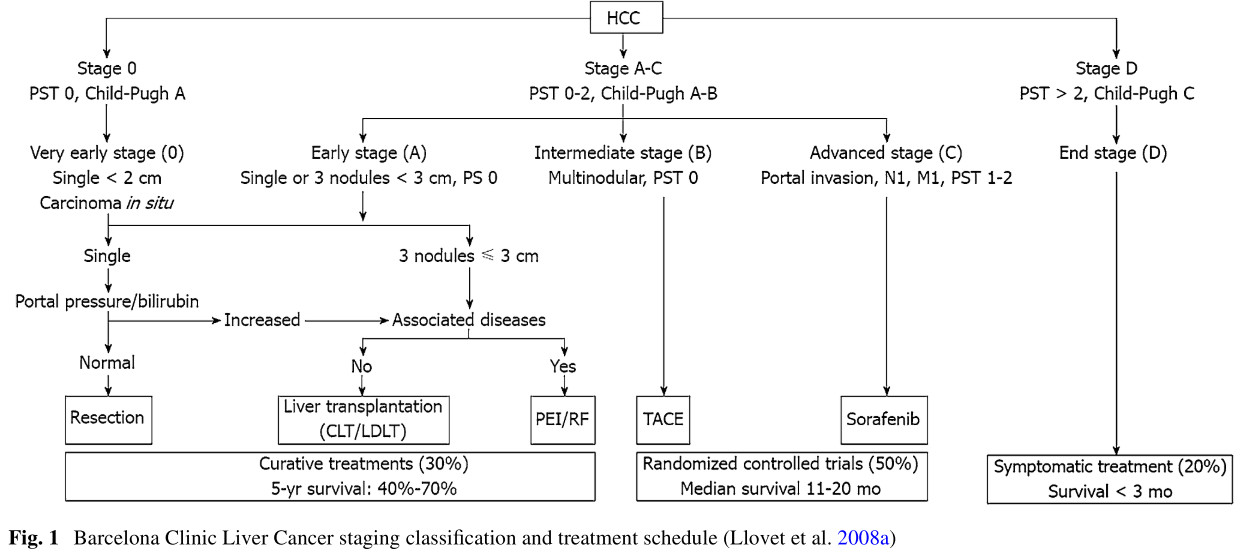
\includegraphics[width=6.26772in,height=2.75000in]{./images/media/image5.png}

These criteria were developed to support previous staging systems such
as the \emph{TNM} as depicted below, that was introduced and refined by
the AJCC, and it incorporated some independent work such as the
\emph{Milan criteria} which concerns only a specific subtype of the
\emph{TNM} staging system {[}\textbf{ref Mazzaferro et al}{]}.

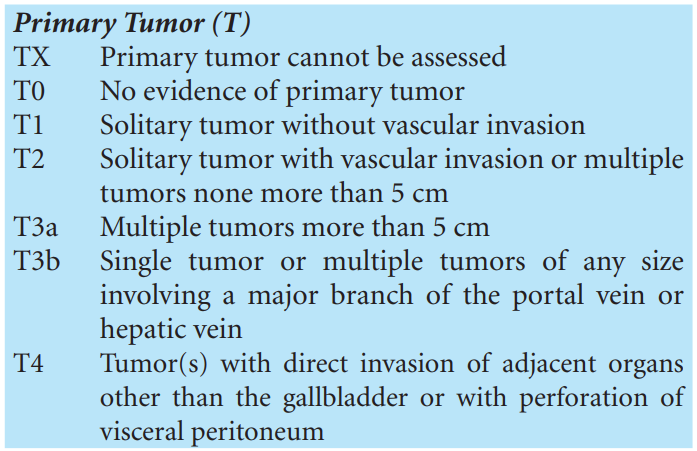
\includegraphics[width=3.53968in,height=2.29099in]{./images/media/image1.png}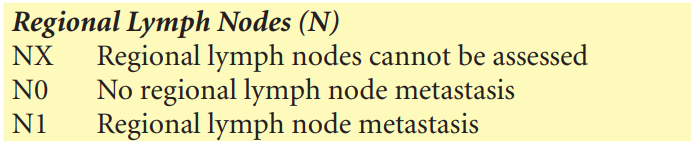
\includegraphics[width=3.54596in,height=0.73629in]{./images/media/image8.png}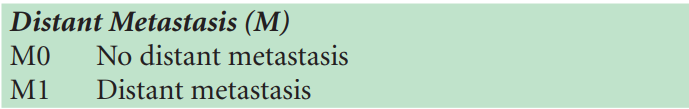
\includegraphics[width=3.55297in,height=0.56068in]{./images/media/image12.png}

One of the main advantages brought by the \emph{BCLC} staging system is
to provide strong guidelines concerning the treatments to follow
depending on the disease progression.

Hereafter, we detail the different treatment techniques available for
patients suffering from \emph{HCCs} when seeking for curation:

\begin{itemize}
\item
  \begin{quote}
  \emph{Surgical resection,} where the best candidates are patients with
  solitary tumor and preserved liver functions {[}\textbf{Fornet et al.
  2018}{]}.\\
  A resection is defined as curative if all macroscopic evidence of
  primary and second tumor are detected in the remnant liver or in any
  other organs by dynamic CT or MR within 4 weeks after surgery
  {[}\textbf{Yang et al. 2012}{]}.\\
  As mentioned by previous studies, resection remains the treatment of
  choice in patients without cirrhosis suffering from HCC. Patients with
  cirrhosis have to be carefully selected to reduce the risk of
  postoperative liver failure {[}\textbf{ref 8, 29, 30 of Breen et al.
  2015}{]}.
  \end{quote}
\item
  \begin{quote}
  \emph{Liver transplantation}, which mainly benefits patients who are
  not good candidates for surgical resection, and fits better those
  within the \emph{Milan criteria} (solitary tumor up to 5cm or less
  than 3 nodules measuring each one less than 3cm) {[}\textbf{Llovet et
  al. 2012 + ref 177}{]}. In theory the transplantation may cure the
  tumor and the underlying cirrhosis at the same time, however, this
  procedure suffers from a scarcity in terms of donors, with an increase
  in the waiting time that led up to 20\% of the potential receivers to
  drop out of the list before finding a donor, even with the existence
  of bridge therapies that can preserve the patient health during the
  waiting time {[}\textbf{ref 161 of Llovet et al.}{]}.\\
  Some modifications have been done to the initial inclusion criteria
  for the transplant candidates after poor recurrence results were
  obtained. {[}\textbf{Llovet et al. 2012}{]}
  \end{quote}
\item
  \begin{quote}
  Image-guided ablation (\emph{IGA}) is the most frequently used
  therapeutic strategy but its efficacy is limited by the size of the
  tumor and its location.\\
  This technique belongs, just like resections, to primary line
  treatments for patients with early stage \emph{HCC} (BCLC stage 0-A)
  for whom surgical management is contraindicated {[}\textbf{Heimbach et
  al. 2017} \textbf{-} \textbf{ref 8 of Breen et al. 2015}{]}. It has
  also been noticed that patients with very small \emph{HCCs} (less than
  2cm in diameter) can benefit from \emph{IGA} to avoid any surgical
  procedure {[}\textbf{ref 9 of Breen et al.}{]}.\\
  Several methods have been developed to perform the destruction of the
  tumor, and radiofrequency ablation (\emph{RFA}) remains the most
  popular technique. Other techniques (thermal or non-thermal) have been
  adopted to overcome limitations of \emph{RFA}.\\
  The risk of complications is higher when the procedure is performed on
  tumors located along the surface of the liver. Indeed, puncture can
  cause bleeding, and heating can cause complications by provoking
  injury on adjacent organs. The intervention should be performed by an
  oncologist with sufficient experience, in order to assess the risk of
  causing damages to the gastrointestinal tract {[}\textbf{ref Breen et
  al.}{]}.\\
  However, \emph{RFA} techniques have recently been improved by the
  assistance of 3D navigation systems, allowing better planning with
  multiple overlapping ablation zones, a more accurate placement of the
  probes and an assessment of the results intraoperatively, thanks to
  image fusion. This new generation of techniques is called
  ``\emph{stereotactic RFA}'' {[}\textbf{Bale et al. 2019, Laimer et al.
  2019 - Perrodin et al. 2019}{]}.\\
  Therefore, the question whether to choose resection over \emph{RFA} is
  still open {[}\textbf{Heimbach et al. 2017 - Bale et al. 2019}{]}.
  \end{quote}
\item
  \begin{quote}
  Transarterial Chemoembolization (\emph{TACE}), which has survival
  benefits in asymptomatic patients with multifocal disease without
  vascular invasion or extrahepatic spread can also be considered
  {[}\textbf{ref Fornet et al. 2018}{]}.\\
  \emph{TACE} can also be applied to patients in earlier stages, who are
  not suitable for the other therapeutic available treatments. This
  clinical situation is known as ``treatment stage migration'' and
  reflects a certain flexibility in the \emph{BCLC} clinical
  interpretation {[}\textbf{Burrel et al, 2012}{]}.
  \end{quote}
\end{itemize}

The same staging systems are used for the patient follow-up, and can be
supported by other metrics such as the \emph{RECIST} (standing for
``\emph{Response evaluation criteria in solid tumours''}) which assess
the tumor response, but presents several limitations and has already
been modified in the past to incorporate changes {[}\textbf{ref
Eisenhauer et al. 2008}{]}.

As explained here, general staging systems rely mainly on the macro
changes caused by the disease, ignoring many histological measurements,
such as the histological grade, depicted below, and defined following
the Edmonson-Steiner grading system, corresponding to the level of
cellular differentiation {[}ref Edmonson 1954{]}:

\begin{itemize}
\item
  \begin{quote}
  G1: Well differentiated
  \end{quote}
\item
  \begin{quote}
  G2: Moderately differentiated
  \end{quote}
\item
  \begin{quote}
  G3: Poorly differentiated
  \end{quote}
\item
  \begin{quote}
  G4: Undifferentiated
  \end{quote}
\end{itemize}

\begin{longtable}[c]{@{}l@{}}
\toprule
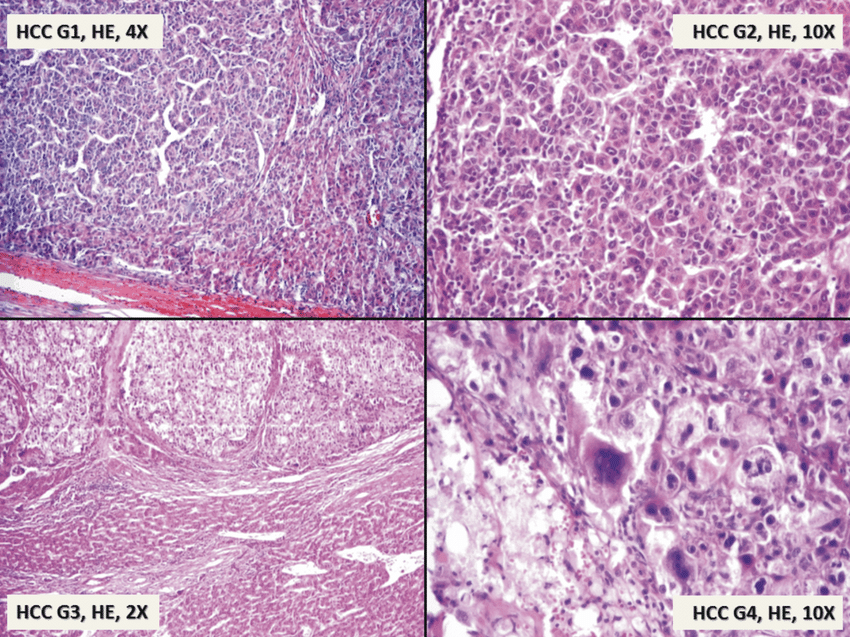
\includegraphics[width=4.14503in,height=3.11935in]{./images/media/image11.png}\tabularnewline
\midrule
\endhead
Histological grades as illustrated by Turdean et al. 2012~{[}ref Turdean
et al. 2012{]}\tabularnewline
\bottomrule
\end{longtable}

Current methods to evaluate the tumor and to propose the best available
treatment still suffer from a lot of limitations, especially because
they rely on subjective interpretation of images, or clinical data, and
also because of the discrete staging systems that are used in a clinical
routine.

The main hypothesis of our research work is that medical images can be
enhanced to provide a subjective feedback to the clinicians, and help
them with non-invasive tools to give to patients suffering from
\emph{HCCs} the best chances of survival.

\emph{(Add a short introduction to radiomics here)*}

\end{document}
